% ============================================================
%  A Lightweight Distributed Anomaly-Based IDS for RPL Networks
%  CPS and IoT Security, UniPD Master CS
% ============================================================
\documentclass[11pt, a4paper]{article}

% --- Encoding & language ------------------------------------
\usepackage[T1]{fontenc}
\usepackage[utf8]{inputenc}
\usepackage[english]{babel}

% --- Page geometry ------------------------------------------
\usepackage[top=2.2cm, bottom=2.2cm, left=2.4cm, right=2.4cm]{geometry}

% --- Typography ---------------------------------------------
\usepackage{microtype}
\usepackage{lmodern}
\usepackage{setspace}
\setstretch{1.05}

% --- Headers & footers --------------------------------------
\usepackage{fancyhdr}
\setlength{\headheight}{13.6pt}
\pagestyle{fancy}
\fancyhf{}
\fancyhead[L]{\small CPS and IoT Security}
\fancyhead[R]{\small Anomaly-Based IDS for RPL}
\fancyfoot[C]{\small \thepage}
\renewcommand{\headrulewidth}{0.4pt}

% --- Section formatting -------------------------------------
\usepackage{titlesec}
\titleformat{\section}{\large\bfseries}{\thesection}{1em}{}
\titleformat{\subsection}{\normalsize\bfseries}{\thesubsection}{1em}{}
\titlespacing*{\section}{0pt}{1.6ex plus 0.3ex}{0.9ex}
\titlespacing*{\subsection}{0pt}{1.3ex plus 0.2ex}{0.6ex}

% --- Graphics, captions, tables -----------------------------
\usepackage{graphicx}
\usepackage{float}
\graphicspath{{img/}}
\usepackage{caption}
\captionsetup{font=small, labelfont=bf, justification=centering,
              skip=4pt, belowskip=2pt}
\usepackage{booktabs}
\usepackage{array}
\usepackage{tabularx}
\usepackage{amsmath}
\usepackage{listings}

% --- Code listings ------------------------------------------
\lstset{
  basicstyle=\ttfamily\scriptsize,
  keywordstyle=\bfseries,
  commentstyle=\itshape,
  language=C,
  showstringspaces=false,
  columns=fullflexible,
  frame=single,
  framesep=3pt,
  xleftmargin=2pt,
  aboveskip=6pt,
  belowskip=4pt
}

% --- Hyperlinks ---------------------------------------------
\usepackage[colorlinks=true, linkcolor=black, urlcolor=blue, citecolor=black]{hyperref}

% --- Miscellaneous ------------------------------------------
\usepackage{parskip}
\setlength{\parskip}{0.6ex plus 0.1ex}
\usepackage{enumitem}
\setlist{noitemsep, topsep=2pt, leftmargin=*}
\usepackage{xcolor}
\usepackage{csquotes}

% ============================================================
\begin{document}

% ---- Title page --------------------------------------------
\begin{titlepage}
  \centering
  
\includegraphics[width=0.32\textwidth]{unipd_logo}

  \vspace{0.4cm}
  {\large\scshape Università degli Studi di Padova}\\[0.1cm]
  {\normalsize Department of Mathematics ``Tullio Levi-Civita''}\\[0.1cm]
  {\normalsize Master's Degree in Computer Science}\\[0.1cm]
  {\normalsize Academic year 2025/2026}

  \vspace{1.1cm}
  \rule{\linewidth}{0.5pt}\\[0.3cm]
  {\LARGE\bfseries CPS and IoT Security}\\[0.4cm]
  {\large A lightweight distributed anomaly-based}\\[0.25cm]
  {\large Intrusion Detection System for}\\[0.25cm]
  {\large RPL networks in Contiki-NG and Cooja}\\[0.2cm]
  \rule{\linewidth}{0.5pt}

  \vspace{0.9cm}
  {\small Reference paper: B. Farzaneh, M. A. Montazeri, S. Jamali,\\
  \textit{An Anomaly-Based IDS for Detecting Attacks in RPL-Based\\
  Internet of Things}, ICWR 2019}

  \vfill
  {\normalsize Author: \textbf{Riccardo Fabbian}}\\[0.2cm]
  {\normalsize Student ID: \textbf{2140711}}\\[0.2cm]
  {\normalsize Period of work: \textbf{September 2026}}
\end{titlepage}

% ============================================================
\section{Introduction and Objective}
% ============================================================

RPL (RFC 6550) is the routing protocol for Low-Power and Lossy Networks. Its security problem is that encryption protects a network from outsiders but not from a node that has already joined: such a node holds valid keys, so every message it sends is legitimate and cryptography cannot distinguish it from an honest one. The only remaining defence is to observe behaviour, which is what the reference paper does.

The paper detects two internal attacks specific to RPL, the \textbf{neighbour attack} and the \textbf{DIS attack}, using a threshold on the number of control messages each node hears from each of its neighbours. Its appeal is that it is genuinely lightweight and fully distributed: no central monitor, no reporting traffic. The authors report a True Positive Rate (TPR) of 100\% with 0\% False Positive Rate (FPR) for the DIS attack, and 94--100\% TPR for the neighbour attack.

This project has two objectives. The first is to \textbf{reproduce} the detector and both attacks on Contiki-NG v5.2 with Cooja, and to run the paper's experimental matrix. The second is an \textbf{original extension}: the paper evaluates its counters once every five minutes, so an attack starting just after an evaluation goes unnoticed for almost a whole window. A second detector mode with a shorter sliding window was implemented to measure what faster detection costs.

% ============================================================
\section{Background and Threat Model}
% ============================================================

RPL organises the network as a tree (a DODAG) rooted at a border router. Each node holds a \textbf{rank}, its distance from the root, and forwards data to a \textbf{preferred parent} of lower rank. Two of the three control messages matter here. A \textbf{DIO} announces a node's identity and rank, and is how the tree is built and maintained. A \textbf{DIS} solicits a DIO, and is normally sent only by a node that has just been switched on.

DIO transmission is paced by the \textbf{Trickle} algorithm: frequent while the network is unstable, then doubling the interval until the network is almost silent. Crucially, \textit{receiving a DIS resets the Trickle timer to its minimum}. These two facts are the basis of everything that follows. Because a converged network is quiet, a node sending many DIOs is a statistical outlier, which is what the detector exploits. Because a DIS resets everyone's timer, a DIS attacker makes honest nodes do the work for it, which is why Section~\ref{sec:results} shows it to be by far the more expensive attack.

The attacker is an \textbf{internal} node that joined legitimately and sends well-formed messages; it does not break link-layer security. In the \textbf{neighbour attack} it floods DIOs, forcing neighbours to reprocess and reconsider parent selection. In the \textbf{DIS attack} it floods solicitations, provoking a storm of DIOs from honest nodes. Every node runs the detector on what its own radio hears, with no cooperation. As in the paper, wormhole, sinkhole, selective-forwarding and rank attacks are out of scope.

% ============================================================
\section{The Reference Model}
% ============================================================

The paper's detector repeats four phases per observation window. \textbf{(I)} Each node counts the DIOs received from every neighbour. \textbf{(II)} At the end of the window it computes the mean $\mu$ and standard deviation $\sigma$ of those counts and derives a threshold $T=\mu+k\sigma$, where the coefficient

\begin{equation}
  k = -5\cdot10^{-5}x^{4} + 0.0037x^{3} - 0.0899x^{2} + 0.9281x - 0.7903
\end{equation}

depends on the number of neighbours $x$. The authors obtained it by simulating attack-free networks, recording for each neighbourhood size the largest deviation occurring naturally, and fitting a curve through those maxima. \textbf{(III)} A neighbour above $T$ is a neighbour attacker; independently, a neighbour whose DIS count exceeds 3 is a DIS attacker, 3 being the maximum the authors ever observed in normal traffic. \textbf{(IV)} A detected neighbour is \textbf{temporarily blocked} for one minute, becoming permanently blocked once a counter of repeated detections exceeds 2. The block is temporary precisely because an honest node may be flagged by accident.

Baseline parameters, reproduced here: 20/30/40 nodes on a 20\,m grid in $100\times100$\,m, UDGM radio with 50\,m transmission and 100\,m interference range, 1 / 20\% / 30\% attackers, CBR UDP traffic, 30-minute runs, attacks starting at 75\,s, 5-minute window, DIS threshold 3, block threshold 2.

% ============================================================
\section{Implementation}
% ============================================================

The system is four Contiki-NG firmwares plus a host-side analysis pipeline, all pinned inside a Docker image (Contiki-NG \texttt{release/v5.2}, commit \texttt{4ccd1a3b}) so that results are reproducible. Cooja runs headless, driven by a control script inside each scenario, which is what makes a matrix of 148 simulations feasible. Simulations use the native \texttt{cooja} mote, which executes 30 simulated minutes of a 40-node network in a few seconds; the Tmote Sky target is used only for the memory measurements of Section~\ref{sec:overhead}.

\subsection{Capturing and Filtering Control Messages}

Contiki-NG registers exactly one handler per ICMPv6 message type, so a second handler cannot be added from application code. A two-line patch to the routing layer, applied automatically at image build time, inserts a hook at the top of the DIS handler and immediately after the sender address becomes available in the DIO handler:

\begin{lstlisting}
if(!ids_rpl_input(RPL_CODE_DIO, &from)) {   /* patch in rpl-icmp6.c */
  goto discard;                             /* blocked neighbour: drop */
}
\end{lstlisting}

This single hook serves both purposes of the design: it is where messages are counted and where blocked neighbours are filtered. Filtering here rather than deleting the neighbour from the routing tables is deliberate: it achieves the intended effect, since a discarded DIS cannot reset a Trickle timer and a discarded DIO cannot make the attacker a parent, without risking corruption of routing state that the routing layer would in any case rebuild from the next message.

\subsection{The Detector}

Each node keeps its own neighbour table, independent of the routing layer's. This is an interpretation: the paper does not say which "neighbour list" it means, and the routing layer only tracks candidate parents whereas the detector must count every node it hears. Both counts are logged so the difference can be inspected. The hook itself is short:

\begin{lstlisting}
int ids_rpl_input(uint8_t code, const uip_ipaddr_t *from) {
  n = lookup(ids_node_id(from), 1);
  if(code == RPL_CODE_DIO) n->dio++; else if(code == RPL_CODE_DIS) n->dis++;
  if(block_state(n) != 0) { n->dropped++; return 0; }   /* filtered */
  return 1;
}
\end{lstlisting}

The ordering is essential and easy to get wrong: \textbf{counting happens before the block is checked}. Were a blocked neighbour to stop being counted, it would appear silent, would never be detected again, and would never reach the permanent block, so the paper's escalation would never fire.

The threshold is evaluated in \textbf{integer arithmetic scaled by 1000}, because the target has no floating-point unit. The polynomial for $k$ is never evaluated on the mote: since the neighbour count is a small integer, all 41 values are precomputed on the host and compiled in as a lookup table costing 82 bytes. The standard deviation uses an exact integer square root, and the variance is obtained from the identity $n^2\sigma^2 = n\sum x_i^2 - (\sum x_i)^2$, which avoids any intermediate rounding:

\begin{lstlisting}
num         = (uint64_t)n * sumsq - (uint64_t)sum * sum;  /* n^2 * variance */
mean_x1000  = (sum * 1000UL) / n;
sigma_x1000 = isqrt64(num * 1000000ULL) / n;
thr_x1000   = mean_x1000 + (k_x1000 * sigma_x1000) / 1000;
\end{lstlisting}

The sliding mode reuses this function unchanged. It differs only in storage and cadence: each neighbour keeps six 10-second buckets in a ring buffer instead of one counter, and the evaluation timer fires every 10 seconds over the rolling 60-second total rather than every 300 seconds. Confining the difference to those two points is what makes the comparison in Section~\ref{sec:sliding} fair, since both modes run identical detection code.

\subsection{Attackers, Logging and Verification}

The attacker firmwares are ordinary nodes plus a timer that calls the routing layer's \textit{own} DIO or DIS transmission functions. Using the protocol's functions rather than crafting packets guarantees the injected messages are indistinguishable from legitimate ones, which is what the threat model requires. Rate, start and duration are build parameters.

Nodes emit tab-separated records over the serial line: one per received message, one per neighbour at each evaluation, one for the computed profile and threshold, one per alert and per blocking action, plus periodic status lines. Attackers additionally log every injection, and the scenario generator writes a separate ground-truth file naming the attackers. \textbf{The analysis joins alerts against that file and never infers ground truth from detector output}, which would make the evaluation circular.

Because the mote arithmetic is hand-written integer code, it is duplicated in Python as a bit-exact reference model. A test replays every stored log, recomputes the profile and alerts from the logged counts, and requires an exact match on every intermediate value. The suite has 28 tests and covers the awkward cases: zero neighbours, one neighbour, identical counts, a single large outlier, and DIS counts exactly at and one above the threshold. Running the same scenario twice produced byte-identical logs, so all variation reported below comes from changing the seed.

% ============================================================
\section{Results and Critical Evaluation}
\label{sec:results}
% ============================================================

The main matrix covers 20/30/40 nodes with 1, 20\% and 30\% attackers, both attacks and both detector modes, over 5 seeds; two sweeps on the DIS threshold and the attack rate use 3 seeds. Figure~\ref{fig:topo} shows the largest configuration, generated from the seed together with its ground-truth file. Node-level metrics classify each node once, matching the paper's table: an attacker is a true positive if any monitor flagged it, a normal node a false positive if any monitor flagged it with the same rule.

\begin{figure}[H]
  \centering
  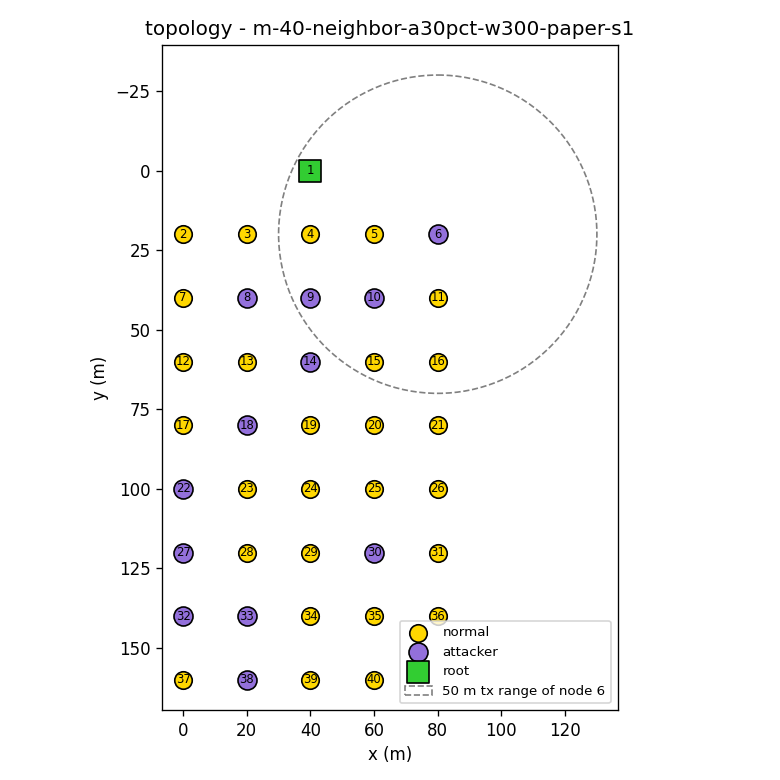
\includegraphics[width=0.46\textwidth]{fig01_topology}
  \caption{The 40-node scenario with 30\% attackers. Root at top centre (green), attackers in purple; the dashed circle is one attacker's 50\,m transmission range}
  \label{fig:topo}
\end{figure}

\subsection{Baseline and the DIS Attack}

Attack-free runs converge within about 60\,s, deliver every datagram, and average one parent change per node. Per-neighbour DIO counts fall from the Trickle burst to 0--1 per window, and the per-neighbour DIS count never exceeded 2, independently confirming the paper's threshold of 3.

\textbf{The DIS attack reproduces the paper exactly}: 100\% TPR and 0\% FPR at every size, every attacker proportion, every seed and both modes. Figure~\ref{fig:dis} shows why the result is so clean rather than merely good: honest nodes stop sending DIS after joining, the attacker never stops, and the two populations do not overlap at all, so a threshold placed between them cannot err in either direction. This is the ideal case for a threshold detector, and it is worth noting that the paper's headline result rests on that separation rather than on the sophistication of the method.

\begin{figure}[H]
  \centering
  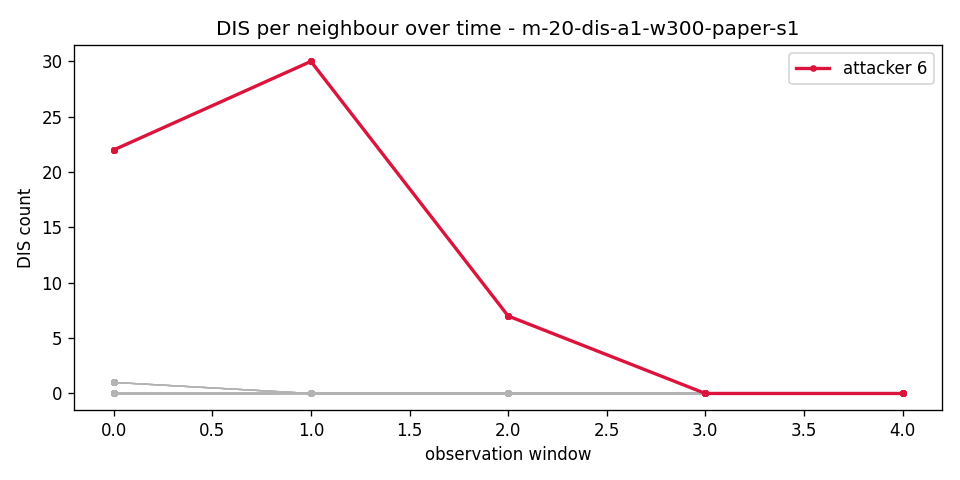
\includegraphics[width=0.86\textwidth]{fig03_dis_over_time}
  \caption{DIS messages per neighbour. Honest nodes stop after joining; the attacker's stream is separated by a wide margin}
  \label{fig:dis}
\end{figure}

\subsection{The Neighbour Attack and Two Structural Findings}

A single neighbour attacker is detected at 100\% TPR. Figure~\ref{fig:threshold} shows the mechanism at a detecting monitor: the attacker's count crosses the dynamic threshold while the neighbourhood mean stays low.

\begin{figure}[H]
  \centering
  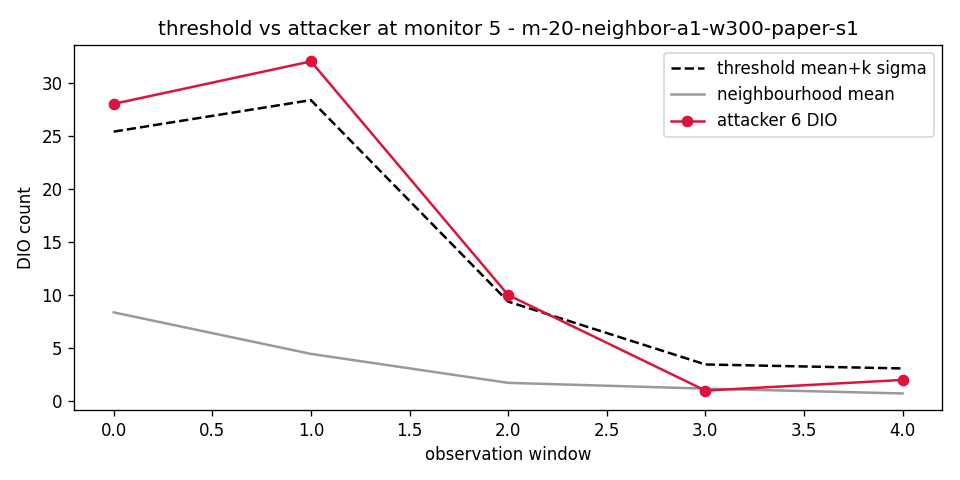
\includegraphics[width=0.78\textwidth]{fig04_threshold_vs_count}
  \caption{Dynamic threshold, neighbourhood mean and the attacker's DIO count at a detecting monitor}
  \label{fig:threshold}
\end{figure}

But TPR \textbf{collapses as the attacker proportion grows}: 100\% with one attacker, 33\% at 20\%, and 5\% at 30\%, against the paper's 94--99\%. This is not an implementation defect, and the analysis of why is the main critical contribution of this work.

\textbf{Finding 1 --- blind spots at certain neighbourhood sizes.} Algorithm 1 divides by the number of neighbours, making it the \textit{population} standard deviation, computed over a set that \textit{includes the attacker}. By Samuelson's inequality no member of a sample of $n$ values can lie further than $\sqrt{n-1}$ standard deviations from the mean, so a lone attacker is detectable only where $\sqrt{n-1}>k(n)$. This is a hard limit independent of attack rate, because every extra message the attacker sends raises the mean and the deviation that define its own threshold. Since $k$ was fitted to maxima that obey the same inequality, the fitted curve runs very close to the bound and crosses it twice: a monitor with 5--7 or 28--32 neighbours can \textit{never} flag a lone attacker. The prediction was confirmed experimentally. An attacker sending 13--14 DIOs per window against a normal rate of about one was heard by exactly three monitors: the one with 8 neighbours flagged it in all seven windows, while those with 5 and 6 neighbours never flagged it once. The distributed design is what rescues the system, since a single non-blind monitor suffices, which is exactly why node-level TPR stays at 100\% while most individual monitors fail.

\textbf{Finding 2 --- attackers mask each other.} When several attackers share a monitor they all inflate the mean and the deviation, so the threshold rises with them and none stands out. This generalises the same inequality to several outliers and explains the collapse at 20\% and 30\%. The measured drop is steeper than the paper's, and two differences plausibly account for the gap: attackers here are placed by seed and often fall within range of one another, and this attacker floods at a fixed rate whereas the paper's rebroadcasts received DIOs, a less synchronised pattern. Neither changes the mechanism, so the conclusion stands as a limit of the published threshold under collusion.

False positives on the neighbour rule are not noise. They are cases where an honest neighbour sent two or three DIOs in a window where others sent zero or one; because the counts are small integers, such a node sits several deviations above a mean below one. This quantisation effect is the whole source of the neighbour-rule FPR, here a few per cent, and very probably of the paper's 0.2--9.6\% as well.

\subsection{Fixed versus Sliding Window}
\label{sec:sliding}

\begin{table}[H]
  \centering \small
  \begin{tabularx}{0.95\textwidth}{llcXcccc}
    \toprule
    \textbf{Nodes} & \textbf{Attack} & \textbf{Att.} & \textbf{Mode} & \textbf{TPR \%} & \textbf{FPR \%} & \textbf{Lat. s} & \textbf{DIO/min} \\
    \midrule
    20 & DIS       & 1    & paper   & 100.0 & 0.0  & 225 & 27.4 \\
    20 & DIS       & 1    & sliding & 100.0 & 0.0  & 45  & 7.1 \\
    30 & DIS       & 20\% & paper   & 100.0 & 0.0  & 225 & 41.9 \\
    30 & DIS       & 20\% & sliding & 100.0 & 0.0  & 45  & 15.3 \\
    40 & DIS       & 30\% & paper   & 100.0 & 0.0  & 225 & 61.0 \\
    40 & DIS       & 30\% & sliding & 100.0 & 0.0  & 15  & 23.6 \\
    \midrule
    20 & neighbour & 1    & paper   & 100.0 & 7.4  & 225 & 6.2 \\
    20 & neighbour & 1    & sliding & 100.0 & 52.6 & 29  & 5.4 \\
    30 & neighbour & 20\% & paper   & 33.3  & 1.7  & 225 & 11.5 \\
    30 & neighbour & 20\% & sliding & 46.7  & 12.5 & 25  & 9.8 \\
    40 & neighbour & 30\% & paper   & 5.0   & 0.0  & 225 & 24.3 \\
    40 & neighbour & 30\% & sliding & 13.3  & 1.4  & 11  & 20.5 \\
    \bottomrule
  \end{tabularx}
  \caption{Main matrix, node-level, mean over 5 seeds. DIO/min is DIO receptions per node per minute; the attack-free baseline is 4.6}
  \label{tab:main}
\end{table}

Both modes share identical counters, thresholds, topologies and seeds; only the evaluation cadence differs. Averaged over the six attack configurations the sliding window cuts mean detection latency from 225\,s to 28\,s, roughly an order of magnitude, while raising mean node-level FPR from 1.5\% to 11.1\% (Figure~\ref{fig:modes}).

\begin{figure}[H]
  \centering
  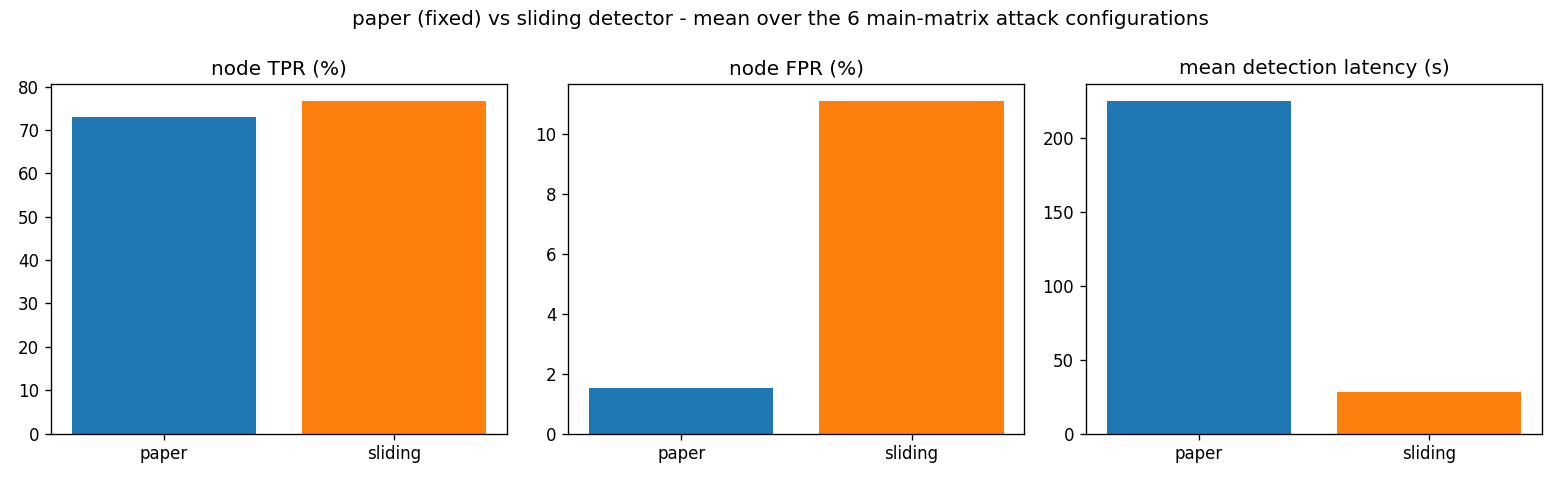
\includegraphics[width=0.94\textwidth]{fig09_mode_comparison}
  \caption{Fixed versus sliding window: detection rate, false-positive rate and mean latency}
  \label{fig:modes}
\end{figure}

Two results were not anticipated. The sliding window \textit{improves} TPR under multiple attackers, from 33\% to 47\% and from 5\% to 13\%, because a shorter window captures an attacker's burst before the other attackers' counts accumulate into the mean; it therefore partly resists the masking of Finding 2. It also halves the traffic the DIS attack provokes, from 61 to 24 DIO receptions per node per minute in the largest configuration, because attackers are blocked earlier and reset far fewer Trickle timers. A faster detector is not only more responsive but cheaper for the network it protects.

The costs are equally concrete, and both are cautionary. In attack-free runs node-level FPR reaches 100\% against 41\%, simply because evaluating thirty times more often gives each honest node thirty times more chances to be flagged once by quantisation. More seriously, the sliding mode issues roughly \textbf{one hundred permanent blocks per run with no attacker present}, against none in the paper mode, because the response parameters (two temporary blocks, then permanent) were calibrated for one decision per five minutes and not for thirty. A sliding detector cannot inherit them unchanged.

\subsection{Sensitivity to Threshold and Attack Rate}

The DIS threshold was tested at 2, 3 and 5: TPR remained 100\% and FPR 0\% in all three, with only the latency rising at 5 (325\,s against 225\,s). Detection is insensitive here because honest nodes never exceed 2 per window and the attacker sends about 10, so any value between separates them. The paper's choice of 3 sits comfortably in the usable range.

The attack-rate sweep (Table~\ref{tab:rates}) produced a \textbf{third finding}. The paper mode detects every rate with the same one-window latency, which is both its strength and its weakness. The sliding mode scales with the attack, down to 5\,s, but \textit{fails completely against a slow DIS attacker}: one message every 30\,s puts at most two inside a 60\,s window, and two never exceeds a threshold of 3 that was calibrated on a window five times longer. The lesson generalises beyond this project: \textbf{a rule expressed as an absolute count is bound to the window that produced it}, and shortening the window silently weakens it. The neighbour rule suffers nothing of the sort because it compares a neighbour against its peers rather than against a fixed number, and it holds at every rate in both modes.

\begin{table}[H]
  \centering \small
  \begin{tabularx}{0.8\textwidth}{lXXX}
    \toprule
    \textbf{Attack} & \textbf{Period} & \textbf{Paper mode} & \textbf{Sliding mode} \\
    \midrule
    DIS       & 1 s            & 100\% / 225 s & 100\% / 5 s \\
    DIS       & 10 s           & 100\% / 225 s & 100\% / 45 s \\
    DIS       & 30 s           & 100\% / 225 s & \textbf{0\%} / not detected \\
    DIS       & random 5--60 s & 100\% / 225 s & \textbf{33\%} / 575 s \\
    neighbour & 1 s            & 100\% / 225 s & 100\% / 5 s \\
    neighbour & 30 s           & 100\% / 225 s & 100\% / 55 s \\
    neighbour & random 5--60 s & 100\% / 225 s & 100\% / 38 s \\
    \bottomrule
  \end{tabularx}
  \caption{TPR / mean latency as a function of attack rate, 20 nodes, one attacker}
  \label{tab:rates}
\end{table}

\subsection{Network Impact and Resource Cost}
\label{sec:overhead}

Packet delivery stayed at 1.000 and end-to-end delay unchanged in \textit{every} configuration, including twelve attackers out of forty. This is a limitation of the setup rather than a property of the attacks: the UDGM radio is configured with success ratio 1.0 and one datagram per node every 30\,s leaves the channel far from saturation, so losses cannot occur. A lossy model would give a less favourable picture. The damage instead falls entirely on the control plane, where it is severe: a single DIS attacker multiplies DIO receptions sixfold and 30\% of attackers thirteenfold (Table~\ref{tab:main}), while parent changes rise from 1.00 to 1.44 per node. On battery-powered devices that translates directly into shortened lifetime. The observation is worth stating plainly: \textit{an attack can be entirely successful while the metric one instinctively checks stays perfect}.

On the Tmote Sky the detector needs 1988\,B of ROM and 588\,B of RAM, the sliding mode adding about 0.5\,kB more for the ring buffers, so the paper's claim of a lightweight module is confirmed. However, under Contiki-NG v5.2 a stock node with only the routing layer and a UDP application already occupies 44578 of 49152\,B of ROM (91\%). The detector fits in the remaining margin but the instrumented firmware used here, which logs every message and decision, exceeds it by about 10\,kB. This is a finding about the platform, not the method: the paper used the same hardware on Contiki 2.7, whose routing layer was much smaller. A deployment carrying the detector without the measurement logging would still fit.

% ============================================================
\section{Conclusion}
% ============================================================

A distributed anomaly-based IDS can detect RPL neighbour and DIS attacks from purely local observations, and the reference model reproduces on a modern stack a decade after publication. The DIS attack is detected at 100\% TPR and 0\% FPR at every size and proportion tested, and a single neighbour attacker is detected reliably, at a cost of about 2\,kB of ROM, 0.6\,kB of RAM and no added traffic.

The reproduction also bounds those claims. Because the threshold computes its dispersion over a set containing the attacker, it can never detect a lone attacker at certain neighbourhood sizes, and it degrades sharply when attackers share a monitor: TPR falls from 100\% to 33\% to 5\% as the attacker proportion rises. Both effects were predicted analytically and then confirmed in simulation, and neither is visible in an evaluation reporting only aggregate rates.

The sliding-window extension shows a clear trade-off: latency falls by an order of magnitude and, unexpectedly, masking resistance improves and the DIS-induced traffic halves; against this, false positives rise sharply, the response parameters over-block the network unless re-derived, and a slow DIS attacker escapes entirely. The last point is the most transferable result of the work: \textbf{the parameters of a threshold detector cannot be separated from the observation window they were measured on}.

Hypotheses H2 (DIS detectable by a fixed threshold), H3 (more attackers degrade detection), H4 (sliding window trades false positives for latency) and H5 (modest, decentralised resource cost) are confirmed. H1 (a neighbour attacker deviates from the DIO profile and is detected) holds only for a single attacker and only outside the blind ranges, and must be qualified accordingly.

% ============================================================
\end{document}
